\documentclass[12pt,a4paper]{article}
\usepackage[utf8]{vietnam}
\usepackage{amsmath,amssymb}
\usepackage{geometry}
\geometry{top=1.5cm,bottom=1.2cm,left=1.4cm,right=1.4cm,headheight=28pt,headsep=12pt,footskip=18pt}
\usepackage{tikz}
\usepackage{xcolor}
\usepackage{enumerate}
\usepackage{graphicx}
\usepackage[version=4]{mhchem}
\usepackage{fancyhdr}
\usepackage{ex_test}

\renewcommand{\baselinestretch}{1.0}
\setlength{\parskip}{1pt}

\definecolor{hfRed}{RGB}{211,47,47}
\definecolor{hfGreen}{RGB}{139,195,144}

\pagestyle{fancy}
\fancyhf{}
\fancyhead[L]{\small\itshape\color{hfRed} Tài liệu lưu hành nội bộ}
\fancyhead[R]{\small\itshape\color{hfRed} Thầy \textbf{TRẦN VĂN THẠNH} - 0777.470.803}
\renewcommand{\headrulewidth}{0.8pt}
\renewcommand{\headrule}{\hbox to\headwidth{\color{hfGreen}\leaders\hrule height \headrulewidth\hfill}}

\fancyfoot[L]{\small\itshape\color{hfRed} CS1: 6/15 Nguyễn Hoàng, P. Kim Long, TP Huế \quad|\quad CS2: 24 Đặng Thái Thân, TP Huế}
\fancyfoot[R]{\small\bfseries\color{hfRed} Trang \thepage}
\renewcommand{\footrulewidth}{0.8pt}
\renewcommand{\footrule}{\hbox to\headwidth{\color{hfGreen}\leaders\hrule height \footrulewidth\hfill}}

\fancypagestyle{firstpage}{
  \fancyhf{}
  \renewcommand{\headrulewidth}{0pt}
  \fancyfoot[L]{\small\itshape\color{hfRed} CS1: 6/15 Nguyễn Hoàng, P. Kim Long, TP Huế \quad|\quad CS2: 24 Đặng Thái Thân, TP Huế}
  \fancyfoot[R]{\small\bfseries\color{hfRed} Trang \thepage}
  \renewcommand{\footrulewidth}{0.8pt}
  \renewcommand{\footrule}{\hbox to\headwidth{\color{hfGreen}\leaders\hrule height \footrulewidth\hfill}}
}

\begin{document}
\thispagestyle{firstpage}

\noindent
\begin{minipage}[t]{0.45\textwidth}
	\centering\fontsize{10pt}{12pt}\selectfont
	\textbf{SỞ GIÁO DỤC VÀ ĐÀO TẠO TP. HUẾ}\\
	\textbf{TRƯỜNG THPT NGUYỄN CHÍ THANH}\\
	\textbf{ĐỀ CHÍNH THỨC}\\
	\textit{(Đề thi có 03 trang)}
\end{minipage}\hfill
\begin{minipage}[t]{0.53\textwidth}
	\centering\small
	\textbf{ĐỀ KIỂM TRA GIỮA HỌC KỲ I -- NĂM HỌC 2025 - 2026}\\
	\textbf{MÔN: HOÁ HỌC. Lớp 11}\\
	\textit{Thời gian làm bài: 45 phút (không kể thời gian phát đề)}\\
	\fbox{\textbf{MÃ ĐỀ: 104}}
\end{minipage}

\smallskip
\noindent\hrulefill
\smallskip

\noindent\textbf{Họ, tên thí sinh:} \dotfill\ \textbf{Lớp:} \dotfill\ \textbf{Số báo danh:} \dotfill

\smallskip
\noindent\textit{(Cho biết nguyên tử khối: H = 1; C = 12; N = 14; O = 16; Na = 23; S = 32; Cl = 35,5; Ba = 137; Al = 27; Cu = 64; Fe = 56).}
\smallskip

\noindent
\textbf{PHẦN I. Câu trắc nghiệm nhiều phương án lựa chọn: (16 câu -- 4 điểm)}\\
\textit{Thí sinh trả lời từ câu 1 đến câu 16. Mỗi câu thí sinh chỉ chọn một phương án.}

\Opensolutionfile{ans}[ans-hoa11-ma104hs]

\begin{ex}
Các dung dịch sau đây có cùng nồng độ 1M, dd nào dẫn điện tốt nhất?
\choice
{$\ce{Ba(OH)2}$}
{$\ce{Al2(SO4)3}$}
{$\ce{H2SO4}$}
{$\ce{NH4NO3}$}
\loigiai{}
\end{ex}

\begin{ex}
Khí thải công nghiệp, khí thải động cơ (ô tô, xe máy ...) là nguyên nhân chủ yếu gây mưa acid. Dãy nào dưới đây gồm các chất có trong các loại khí thải này và là nguyên nhân trực tiếp gây mưa acid?
\choice
{$\ce{SO2}, \ce{CO}, \ce{NO}$.}
{$\ce{NO2}, \ce{CO2}, \ce{CO}$.}
{$\ce{NO}, \ce{NO2}, \ce{SO2}$.}
{$\ce{SO2}, \ce{CO}, \ce{NO2}$.}
\loigiai{}
\end{ex}

\begin{ex}
Cho các phản ứng sau:\\
(1) $\ce{N2 + O2 ->[t^\circ, xt] 2NO}$;\\
(2) $\ce{N2 + 3H2 <=>[t^\circ, xt] 2NH3}$.\\
Trong hai phản ứng trên thì nitrogen
\choice
{thể hiện tính khử và tính oxi hóa.}
{không thể hiện tính khử và tính oxi hóa.}
{chỉ thể hiện tính oxi hóa.}
{chỉ thể hiện tính khử.}
\loigiai{}
\end{ex}

\begin{ex}
Nhận xét nào sau đây \textbf{không đúng}?
\choice
{Phản ứng một chiều là phản ứng luôn xảy ra không hoàn toàn.}
{Trong phản ứng thuận nghịch, các chất sản phẩm có thể phản ứng với nhau để tạo thành chất đầu.}
{Trong phản ứng một chiều, các chất sản phẩm không phản ứng được với nhau tạo thành chất đầu.}
{Phản ứng thuận nghịch là phản ứng xảy ra theo hai chiều trái ngược nhau trong cùng điều kiện.}
\loigiai{}
\end{ex}

\begin{ex}
Trong y học, vì sao nitrogen lỏng được dùng để bảo quản mẫu vật?
\choice
{Do nitrogen hóa lỏng ở nhiệt độ thấp.}
{Do nitrogen không duy trì sự hô hấp.}
{Do nitrogen tan ít rất trong nước.}
{Do nitrogen là chất khí không màu, không mùi, không vị.}
\loigiai{}
\end{ex}

\begin{ex}
Chất nào sau đây là chất điện li?
\choice
{Glucose.}
{Saccharose.}
{Sodium hydroxide.}
{Alcohol ethylic.}
\loigiai{}
\end{ex}

\begin{ex}
Cho $m$ gam Na vào nước dư thu được $1{,}5\text{ L}$ dung dịch có $\text{pH} = 12$. Giá trị của $m$ là
\choice
{$0{,}23\text{ gam}$.}
{$0{,}46\text{ gam}$.}
{$0{,}115\text{ gam}$.}
{$0{,}345\text{ gam}$.}
\loigiai{}
\end{ex}

\begin{ex}
Chuẩn độ dung dịch $\ce{NaOH}$ chưa biết chính xác nồng độ (biết nồng độ trong khoảng gần với $0{,}1\text{ M}$) bằng dung dịch $\ce{HCl}\ 0{,}1\text{ M}$ với chỉ thị phenolphtalein. Chất đóng vai trò là dung dịch chuẩn là?
\choice
{Phenolphtalein.}
{$\ce{NaCl}$.}
{$\ce{NaOH}$.}
{$\ce{HCl}$.}
\loigiai{}
\end{ex}

\begin{ex}
Để hạn chế hiện tượng phú dưỡng, ta có thể dùng bao nhiêu biện pháp sau đây?\\
(1) Tạo điều kiện để nước trong kênh, rạch, ao, hồ được lưu thông.\\
(2) Xử lí nước thải trước khi chảy vào kênh rạch ao hồ.\\
(3) Sử dụng phân bón đúng lượng, đúng cách \& đúng thời điểm.
\choice
{1.}
{2.}
{0.}
{3.}
\loigiai{}
\end{ex}

\begin{ex}
Trong phản ứng tổng hợp $\ce{NH3}$ theo quá trình Haber hỗn hợp $\ce{N2}$ \& $\ce{H2}$ (tỉ lệ mol $x : y$) được nén ở áp suất cao và đưa vào tháp tổng hợp ammonia trong điều kiện nhiệt độ, áp suất và chất xúc tác thích hợp. Tỉ lệ mol $x : y$ là?
\choice
{$1 : 2$.}
{$2 : 1$.}
{$1 : 3$.}
{$3 : 1$.}
\loigiai{}
\end{ex}

\begin{ex}
Xét cân bằng:\\
(1) $\ce{H2(g) + I2(g) <=> 2HI(g)} \quad (K_1)$\\
(2) $\ce{2HI(g) <=> H2(g) + I2(g)} \quad (K_2)$\\
Mối quan hệ giữa $K_1$ và $K_2$ là:
\choice
{$K_1 = 2K_2$.}
{$K_1 = K_2$.}
{$K_1 = \sqrt{K_2}$.}
{$K_1 = K_2^{-1}$.}
\loigiai{}
\end{ex}

\begin{ex}
Công thức Lewis của $\ce{NH3}$ là:
\begin{center}
	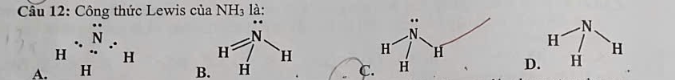
\includegraphics[width=0.6\textwidth]{images_crop/de104_cau12_lewis.png}
\end{center}
\choice
{Công thức A}
{Công thức B}
{Công thức C}
{Công thức D}
\loigiai{}
\end{ex}

\begin{ex}
Kim loại không bị hòa tan trong dung dịch acid $\ce{HNO3}$ đặc nguội, nhưng tan được trong dung dịch $\ce{NaOH}$ là:
\choice
{$\ce{Mg}$}
{$\ce{Al}$}
{$\ce{Fe}$}
{$\ce{Pb}$}
\loigiai{}
\end{ex}

\begin{ex}
Cân bằng hoá học là một trạng thái của phản ứng thuận nghịch tại đó:
\choice
{tốc độ phản ứng thuận bằng một nửa tốc độ phản ứng nghịch.}
{tốc độ phản ứng không thay đổi.}
{tốc độ phản ứng thuận bằng hai lần tốc độ phản ứng nghịch.}
{tốc độ phản ứng thuận bằng tốc độ phản ứng nghịch.}
\loigiai{}
\end{ex}

\begin{ex}
Tổng hệ số (các số nguyên, tối giản) của tất cả các chất trong phương trình phản ứng giữa Cu với dung dịch $\ce{HNO3}$ đặc là
\choice
{11.}
{9.}
{10.}
{8.}
\loigiai{}
\end{ex}

\begin{ex}
Có thể phân biệt muối ammonium với các muối khác bằng cách cho nó tác dụng với dung dịch kiềm đun nóng, vì
\choice
{thoát ra một chất khí màu nâu đỏ, làm xanh giấy quỳ tím ẩm.}
{thoát ra một chất khí màu lục nhạt.}
{thoát ra chất khí không màu, không mùi.}
{thoát ra một chất khí không màu, mùi khai, làm xanh giấy quỳ tím ẩm.}
\loigiai{}
\end{ex}

\Closesolutionfile{ans}

\bigskip
\noindent
\textbf{PHẦN II. Câu trắc nghiệm đúng sai: (2 câu -- 2 điểm)}\\
\textit{Thí sinh trả lời từ câu 1 đến câu 2. Trong mỗi ý a), b), c), d) ở mỗi câu thí sinh chọn đúng hoặc sai.}

\begin{ex}
Hiện tượng phú dưỡng là một biểu hiện của môi trường ao, hồ bị ô nhiễm do dư thừa các chất dinh dưỡng.
\choiceTF
{a) Chất thải công nghiệp, chất thải sinh hoạt, ... khi không được xử lí theo quy chuẩn, nếu thải vào sông, hồ cũng gây ra hiện tượng phú dưỡng.}
{b) Thông thường, khi hàm lượng calcium trong nước đạt $300\ \mu\text{g/L}$ và hàm lượng magnesium đạt $20\ \mu\text{g/L}$ sẽ gây hiện tượng phú dưỡng.}
{c) Có thể quan sát được hiện tượng phú dưỡng thông qua sự xuất hiện dày đặc của tảo xanh trong nước.}
{d) Hiện tượng phú dưỡng gây cản trở hấp thụ ánh sáng mặt trời vào nước, làm giảm sự quang hợp của thực vật thủy sinh.}
\loigiai{}
\end{ex}

\begin{ex}
Cho đồ thị:
\begin{center}
	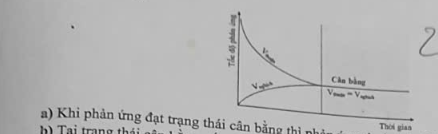
\includegraphics[width=0.45\textwidth]{images_crop/de104_do_thi_can_bang.png}
\end{center}
\choiceTF
{a) Khi phản ứng đạt trạng thái cân bằng thì phản ứng thuận và phản ứng nghịch dừng lại.}
{b) Tại trạng thái cân bằng, tốc độ phản ứng thuận bằng tốc độ phản ứng nghịch.}
{c) Đồ thị trên biểu diễn tốc độ của phản ứng một chiều phụ thuộc vào thời gian.}
{d) Khi phản ứng thuận nghịch xảy ra thì tốc độ phản ứng thuận tăng dần còn tốc độ phản ứng nghịch giảm dần.}
\loigiai{}
\end{ex}

\bigskip
\noindent
\textbf{PHẦN III. Câu trắc nghiệm trả lời ngắn: (4 câu -- 1 điểm)}\\
\textit{Thí sinh trả lời từ câu 1 đến câu 4.}

\begin{ex}
Cho dung dịch $\ce{HNO3}$ tác dụng với các chất sau: $\ce{NH3}, \ce{CaCO3}, \ce{Ag}, \ce{NaOH}$. Có bao nhiêu phản ứng trong đó $\ce{HNO3}$ đóng vai trò acid theo Bronsted?
\shortans{}
\loigiai{}
\end{ex}

\begin{ex}
Nhiệt phân các muối ammonium: $\ce{NH4Cl}, \ce{(NH4)2CO3}, \ce{NH4NO2}, \ce{NH4HCO3}, \ce{NH4NO3}$. Có bao nhiêu trường hợp thu được khí $\ce{NH3}$?
\shortans{}
\loigiai{}
\end{ex}

\begin{ex}
Cho các chất (phân tử và ion): $\ce{NaOH}, \ce{H2S}, \ce{NH3}, \ce{CO3^{2-}}, \ce{S^{2-}}, \ce{NH4+}, \ce{PO4^{3-}}$. Theo quan điểm của Bronsted -- Lowry có bao nhiêu chất có thể là base?
\shortans{}
\loigiai{}
\end{ex}

\begin{ex}
Cho cân bằng hóa học (trong bình kín) sau:
\[ \ce{N2(g) + 3H2(g) <=>[xt, t^\circ, p] 2NH3(g)} \quad \Delta_r H_{298}^\circ = -92\text{ kJ} \]
Trong các yếu tố: (1) Thêm một lượng $\ce{N2}$ hoặc $\ce{H2}$; (2) Thêm một lượng $\ce{NH3}$; (3) Tăng nhiệt độ của phản ứng; (4) Tăng áp suất của phản ứng; (5) Dùng thêm chất xúc tác. Có bao nhiêu yếu tố làm cho tỉ khối của hỗn hợp khí trong bình so với $\ce{H2}$ tăng lên?
\shortans{}
\loigiai{}
\end{ex}

\bigskip
\noindent
\textbf{PHẦN IV. TỰ LUẬN: (3 câu -- 3 điểm)}\\
\textit{Thí sinh trả lời từ câu 1 đến câu 3.}

\begin{ex}
\textbf{(1,0 điểm)} Viết biểu thức tính hằng số cân bằng ($K_C$) cho các phản ứng thuận nghịch sau:
\begin{enumerate}[(1)]
	\item $\ce{H2(g) + F2(g) <=> 2HF(g)}$
	\item $\ce{Fe2O3(s) + 3CO(g) <=> 2Fe(s) + 3CO2(g)}$
\end{enumerate}
\loigiai{}
\vspace*{3.5cm}
\end{ex}

\begin{ex}
\textbf{(1,0 điểm)} Trộn lẫn $V\text{ mL}$ dung dịch $\ce{NaOH}\ 0{,}03\text{ M}$ với $V\text{ mL}$ dung dịch $\ce{HCl}\ 0{,}01\text{ M}$ được $2V\text{ mL}$ dung dịch Y. Dung dịch Y có pH là bao nhiêu?
\loigiai{}
\vspace*{4.5cm}
\end{ex}

\begin{ex}
\textbf{(1,0 điểm)} Nước cường toan trong tiếng Anh là Aqua Regia (nghĩa là nước hoàng gia) -- là hợp chất có tính ăn mòn mạnh, ở dạng lỏng, có màu vàng và dễ bay hơi, được sử dụng cho 1 số quy trình hóa học phân tích và để tinh chế vàng. Hãy nêu thành phần của nước cường toan và viết phản ứng của nước cường toan với vàng.
\loigiai{}
\vspace*{4.5cm}
\end{ex}

\begin{center}
\textbf{--------- HẾT ---------}\\
\textit{(Học sinh không sử dụng tài liệu và bảng tuần hoàn hoá học)}
\end{center}

\end{document}
